\section{Постановка задачи}

В таблице ниже приводятся сведения об уровне среднегодовых цен на говядину из США на рынках Нью-Йорка:

\VerbatimInput{figures/table.txt}

Необходимо проверить гипотезу о нормальном распределении на уровне значимости 5\% и 10\% первых разностей по критериям Колмогорова и $\omega^2$ для сложных гипотез.

\section{Ход работы}

Изначально был изучен раздел 2.2.4 из книги Буре В.М., Парилина Е.М., Седаков А.А. <<Методы прикладной статистики в R и Excel>>.

Перед проверкой гипотез необходимо провести предварительные вычисления над данными. Сначала были найдены первые разности изначальных данных. Затем из этих разностей были исключены все повторения, которые могли в дальнейшем повлиять на вычисления, а также полученная выборка была отсортирована. Полученный вариационный ряд с некоторыми характеристиками представлен в конце файла. График полученной эмпирической функции представлен ниже.

\begin{figure}[H]
	\begin{minipage}[H]{\linewidth}
		\begin{center}
			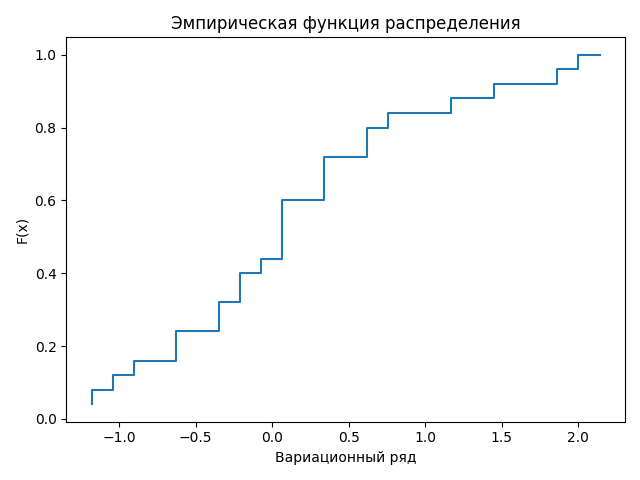
\includegraphics[width=\linewidth]{figures/ecdf}
		\end{center}
	\end{minipage}
\end{figure}

Дальнейшие вычисления по критериям производились в соответствии с алгоритмами, описывающие критерии.

\subsection{Выборочные характеристики}

Изначально было сгенерировано две выборки объёмом 60 и 80 значений из нормально распределённых генеральных совокупностей с разными случайными значениями параметров математического ожидания и среднеквадратического отклонения. Их этих двух выборок была сформирована обобщённая выборка (объёмом 140 значений), которая была упорядочена по возрастанию её значений с помощью сортировки.

Вручную были получены основные выборочные характеристики. Коэффициент вариации составляет 385\%, что говорит о большом разбросе значений и, как следствие, о неднородности выборки. Коэффициент асимметрии достаточно близок к нулю, что говорит о не большом отклонении от пика распределения (математического ожидания). Коэффициент эксцесса показывает, что данное распределение обладает более пологим пиком, чем эмпирическое.

Сгенерированная выборка и полученные выборочные характеристики представлены в конце отчёта.

Было произведено разбиение размаха выборки на конечное число непересекающихся интервалов. Число интервалов разбиения, согласно постановке задачи, производилось по следующим величинам:

\begin{itemize}
	\item $r = 10$;
	\item $r = 20$;
	\item $r = 30$;
	\item $r = [ 1 + 3.2 \lg{n} ]$, где $n$ - объём выборки.
\end{itemize}

Таким образом, для каждого $r$ были построены:

\newpage
\begin{itemize}
	\item Гистограмма частот распределения;
	
	\begin{figure}[H]
		\begin{minipage}[H]{0.44\linewidth}
			\center{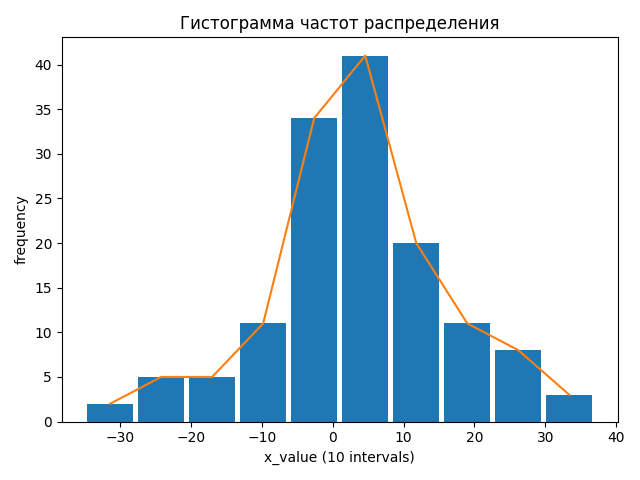
\includegraphics[width=\linewidth]{figures/freq_hist_10_bins}}
		\end{minipage}
		\hfill
		\begin{minipage}[H]{0.44\linewidth}
			\center{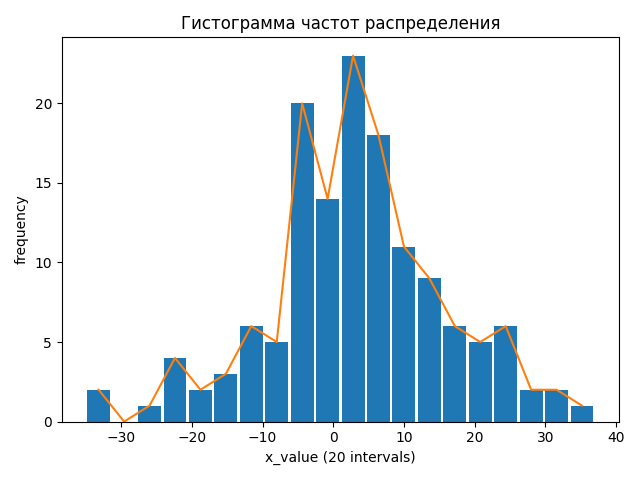
\includegraphics[width=\linewidth]{figures/freq_hist_20_bins}}
		\end{minipage}
		\vfill
		\begin{minipage}[H]{0.44\linewidth}
			\center{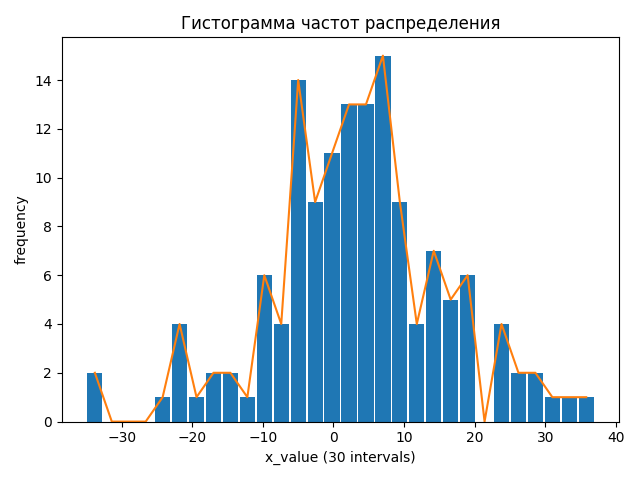
\includegraphics[width=\linewidth]{figures/freq_hist_30_bins}}
		\end{minipage}
		\hfill
		\begin{minipage}[H]{0.44\linewidth}
			\center{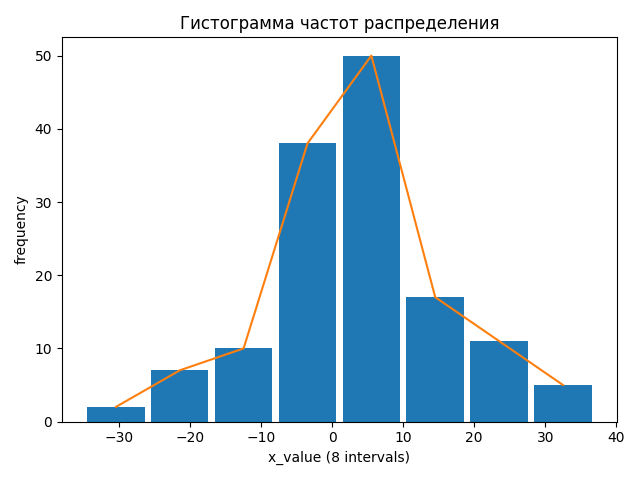
\includegraphics[width=\linewidth]{figures/freq_hist_8_bins}}
		\end{minipage}
	\end{figure}
	
	\item Гистограмма распределения частот и график интегральных частот;
	
	\begin{figure}[H]
		\begin{minipage}[H]{0.44\linewidth}
			\center{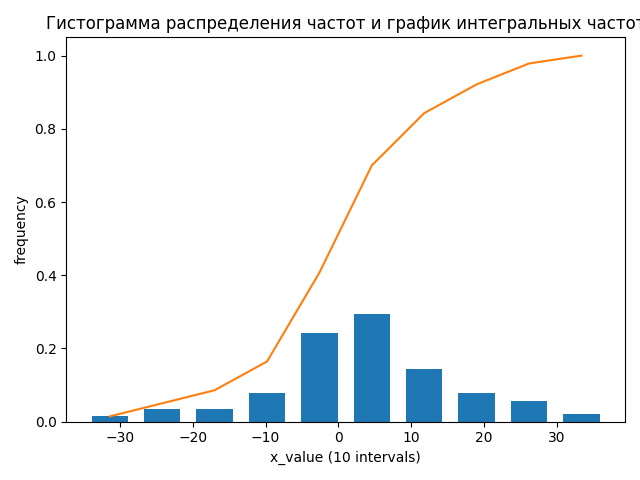
\includegraphics[width=\linewidth]{figures/freq_hist_cum_freq_10_bins}}
		\end{minipage}
		\hfill
		\begin{minipage}[H]{0.44\linewidth}
			\center{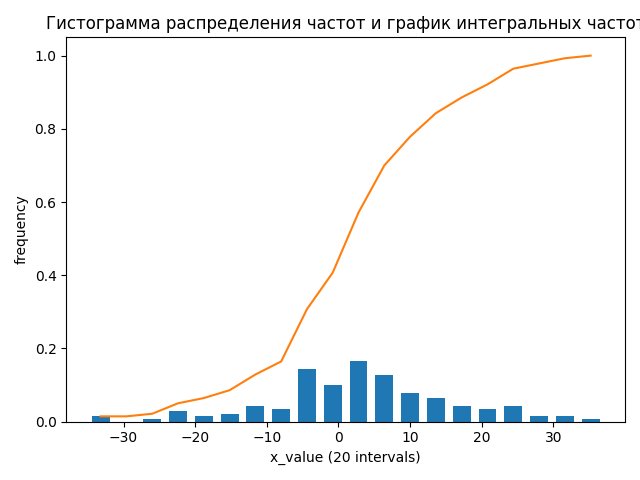
\includegraphics[width=\linewidth]{figures/freq_hist_cum_freq_20_bins}}
		\end{minipage}
		\vfill
		\begin{minipage}[H]{0.44\linewidth}
			\center{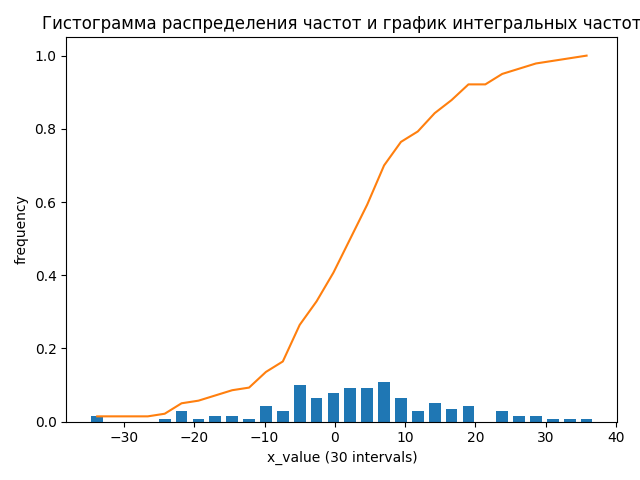
\includegraphics[width=\linewidth]{figures/freq_hist_cum_freq_30_bins}}
		\end{minipage}
		\hfill
		\begin{minipage}[H]{0.44\linewidth}
			\center{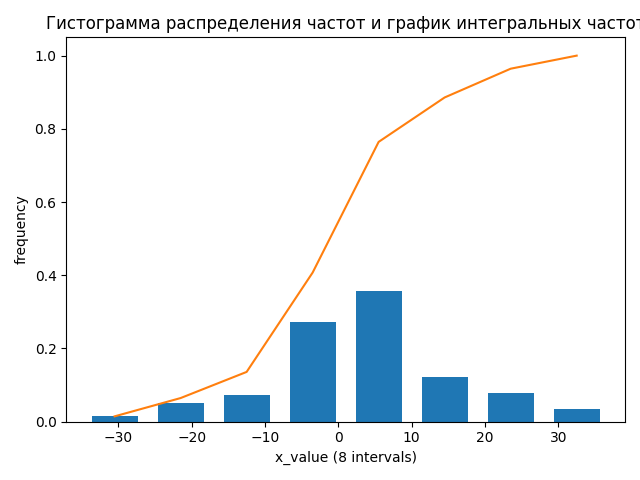
\includegraphics[width=\linewidth]{figures/freq_hist_cum_freq_8_bins}}
		\end{minipage}
	\end{figure}
	
	\item Гистограмма относительных кумулятивных частот;
	
	\begin{figure}[H]
		\begin{minipage}[H]{0.44\linewidth}
			\center{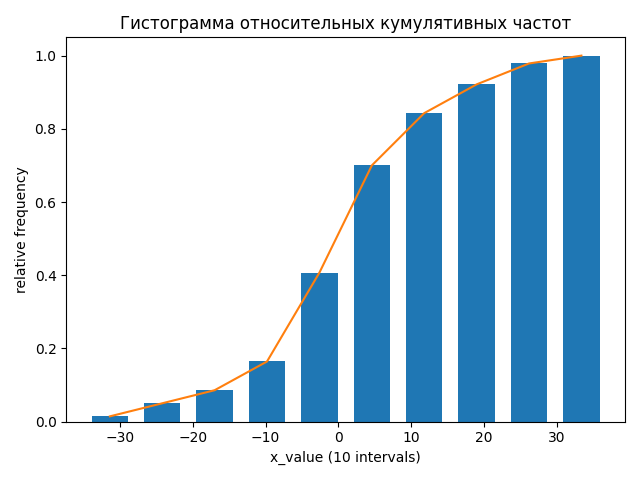
\includegraphics[width=\linewidth]{figures/rel_cum_hist_10_bins}}
		\end{minipage}
		\hfill
		\begin{minipage}[H]{0.44\linewidth}
			\center{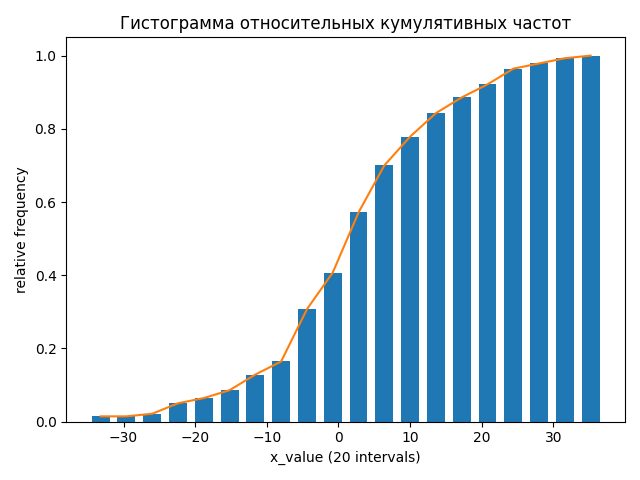
\includegraphics[width=\linewidth]{figures/rel_cum_hist_20_bins}}
		\end{minipage}
		\vfill
		\begin{minipage}[H]{0.44\linewidth}
			\center{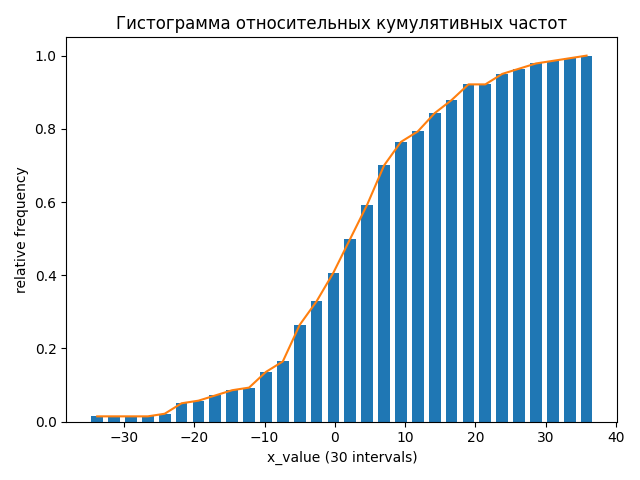
\includegraphics[width=\linewidth]{figures/rel_cum_hist_30_bins}}
		\end{minipage}
		\hfill
		\begin{minipage}[H]{0.44\linewidth}
			\center{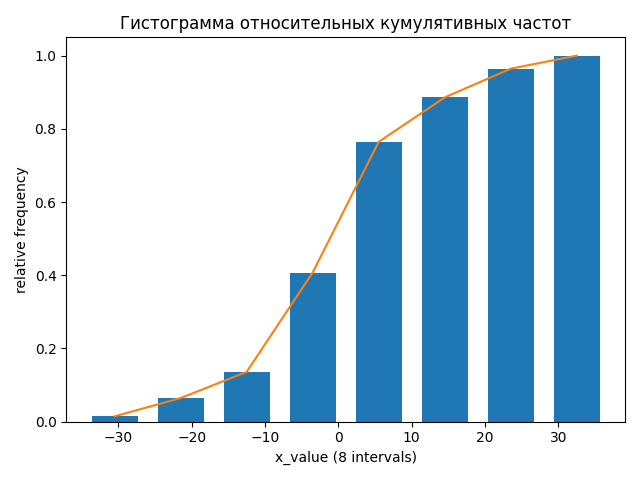
\includegraphics[width=\linewidth]{figures/rel_cum_hist_8_bins}}
		\end{minipage}
	\end{figure}
	
	\item Гистограмма плотности относительных частот;
	
	\begin{figure}[H]
		\begin{minipage}[H]{0.44\linewidth}
			\center{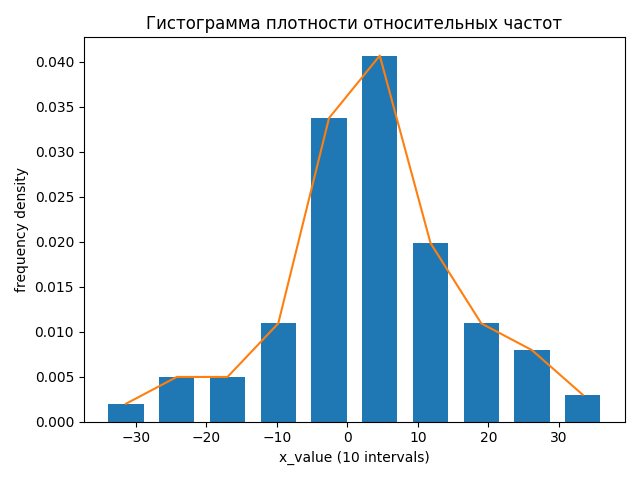
\includegraphics[width=\linewidth]{figures/rel_den_hist_10_bins}}
		\end{minipage}
		\hfill
		\begin{minipage}[H]{0.44\linewidth}
			\center{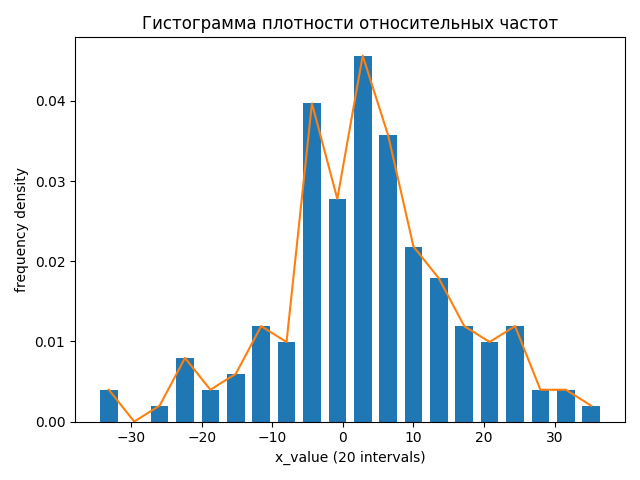
\includegraphics[width=\linewidth]{figures/rel_den_hist_20_bins}}
		\end{minipage}
		\vfill
		\begin{minipage}[H]{0.44\linewidth}
			\center{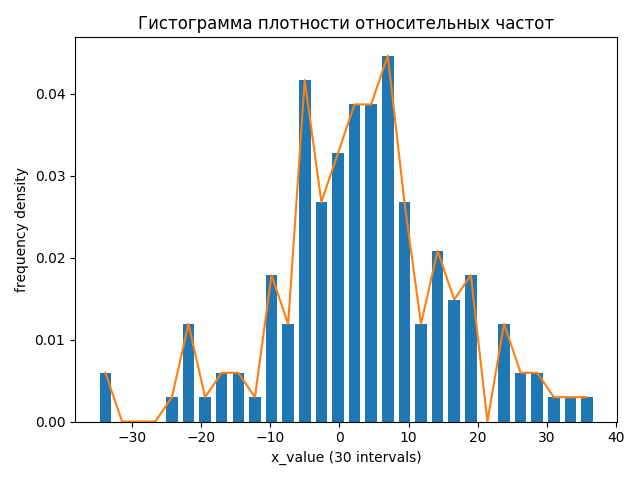
\includegraphics[width=\linewidth]{figures/rel_den_hist_30_bins}}
		\end{minipage}
		\hfill
		\begin{minipage}[H]{0.44\linewidth}
			\center{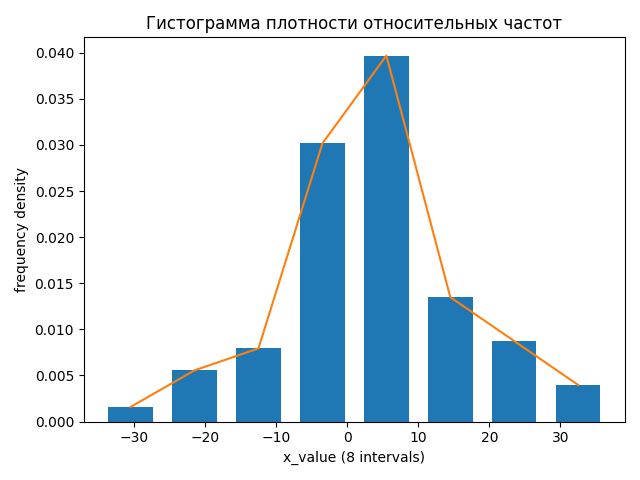
\includegraphics[width=\linewidth]{figures/rel_den_hist_8_bins}}
		\end{minipage}
	\end{figure}
	
	\item Гистограмма относительных частот.
	
	\begin{figure}[H]
		\begin{minipage}[H]{0.44\linewidth}
			\center{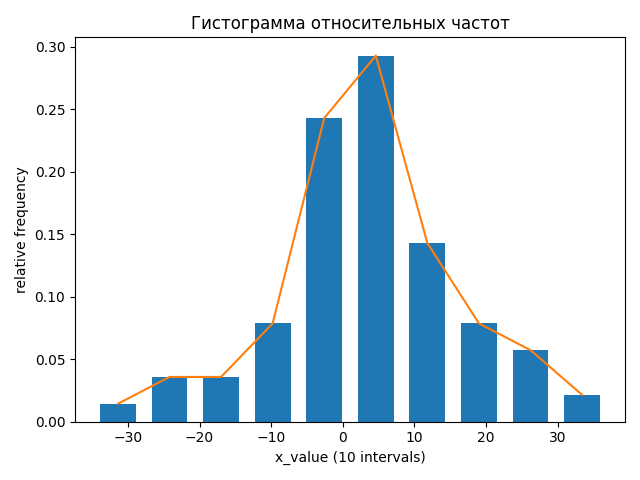
\includegraphics[width=\linewidth]{figures/rel_freq_hist_10_bins}}
		\end{minipage}
		\hfill
		\begin{minipage}[H]{0.44\linewidth}
			\center{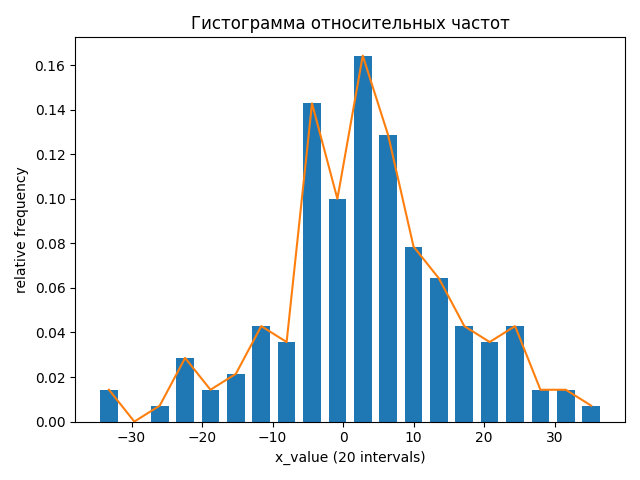
\includegraphics[width=\linewidth]{figures/rel_freq_hist_20_bins}}
		\end{minipage}
		\vfill
		\begin{minipage}[H]{0.44\linewidth}
			\center{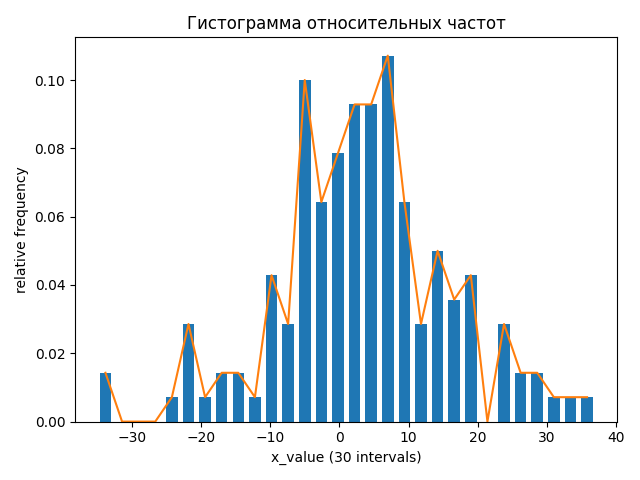
\includegraphics[width=\linewidth]{figures/rel_freq_hist_30_bins}}
		\end{minipage}
		\hfill
		\begin{minipage}[H]{0.44\linewidth}
			\center{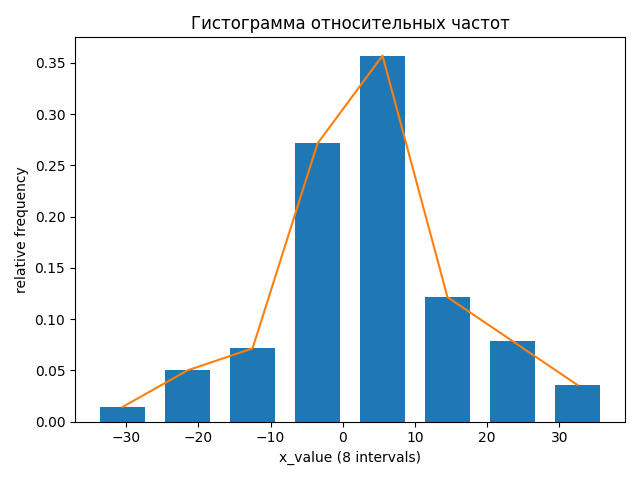
\includegraphics[width=\linewidth]{figures/rel_freq_hist_8_bins}}
		\end{minipage}
	\end{figure}
	
\end{itemize}

При малых интервалах разбиения ($r = 8, r = 10 $) нельзя утверждать о неоднородности выборки, однако при увеличении числа интервалов становится явно видно 2 пика, которые и могут послужить аргументом для утверждения неоднородности выборки. Исходя из дескриптивной статистики, можно также сделать вывод о наличии существенной неоднородности в исходных данных.

Таким образом, в ходе работы были вычислены основные статистические характеристики, построены гистограммы, полигоны плотности и кумулятивные частоты и на основе всего вышеперечисленного сделаны выводы.

\subsection{Критерий $\omega^2$}

\textit{Алгоритм критерия $\omega^2$ в случае сложной гипотезы о нормальности распределения генеральной совокупности}

\begin{enumerate}
	\item Выдвинуть нулевую гипотезу $H_0: F_{\xi}(\cdot) = F_0(\cdot, \theta)$. Сформулировать альтернативную гипотезу $H_1: F_{\xi}(\cdot) \ne F_0(\cdot, \theta)$;
	\item Задать уровень значимости критерия $\alpha$;
	\item Найти оценки $\hat{\theta} = (\overline{x}, s^2)$ неизвестных параметров распределения $\theta = (a, \sigma^2)$;
	\item Вычислить значение исправленной формы статистики $\hat{\omega}^2_n$ следующим образом:
	\begin{enumerate}
		\item По выборке $X_{[n]}$ построить эмпирическую функцию распределения $F_n(x)$ по формуле (\ref{ecdf})
		\item Определить $\omega^2_n$ по формуле 
		
		\begin{equation}
			\omega^2_n = \frac{1}{12n} + \sum\limits_{i=1}^n \left(F_0(x_i) - \frac{2i - 1}{2n} \right)^2
		\end{equation}
		
		\item Вычислить значение исправленной формы модифицированной статистики $\omega^2$ по формуле
		
		\begin{equation}
			\hat{\omega}^2_n = \omega^2_n \left(1 + \frac{0.5}{n} \right)
		\end{equation}
		
	\end{enumerate}
	
	\item Найти критическую область - интервал $(w_{1-\alpha}; \infty)$. Квантиль $w_{1 - \alpha}$ можно найти из таблицы ниже
	
	\begin{center}
		\begin{tabular}{|c|c|c|c|c|c|}
			\hline
			Модифицированная форма & 0.15 & 0.1 & 0.05 & 0.025 & 0.01 \\
			\hline
			$\omega^2_n \left(1 + \frac{0.5}{n} \right)$ & 0.091 & 0.104 & 0.126 & 0.148 & 0.178 \\
			\hline
		\end{tabular}
	\end{center}
	
	\item Если численное значение статистики $\hat{\omega}^2_n$ попадает в интервал $(w_{1 - \alpha}; \infty)$, то нулевая гипотеза $H_0$ отвергается, в противном случае нет оснований отвергнуть нулевую гипотезу при уровне значимости приближённо равном $\alpha$.
	
\end{enumerate}

Результаты работы данного критерия представлены ниже.

\VerbatimInput{figures/file.txt}
